%!TEX program = xelatex
%!TEX root = ./thesis.tex
\chapter{Methodology}
%!TEX program = xelatex
%!TEX root = ./thesis.tex
\section{Target Environments}\label{sec_env}
\subsection{Summary of Environment Design}
We propose and develop a set of tasks that are representatives of deep reinforcement learning environments with continuous action space, multi-modal state space and sparse reward functions. The design of the robots' physical systems is based on the 3D robot environments~\cite{roboschool_2018} in OpenAI Gym~\cite{openaigym}. The external environments and reward functions of the target tasks are different from the original environments in OpenAI Gym. There are three classes of 3D robot agents in the environments OpenAI Gym: Ant, Humanoid and Swimmer. The Ant agent is a quadruped robot with 8-dimensional action space, the Humanoid agent is a humanoid robot with 16-dimensional action space, and the Swimmer agent is a worm-like robot with 2-dimensional action space.  The three agents are shown in Figure~\ref{fig_agent_ant}, Figure~\ref{fig_agent_humanoid} and Figure~\ref{fig_agent_swimmer}.

We mainly focus on a set of different problems based on the Ant agent, because the agent has the capability of solving a rich variety of high-level tasks, while the learning of the agent's basic control skills is not too challenging. 
Compared to the Ant agent, the Swimmer agent is too simple and its capability of solving hierarchical tasks is limited. The Humanoid agent, on the other hand, has a much more unstable physical system compared to Ant, and poses too much difficulty in the learning basic locomotion skills.
\begin{figure}[H]
	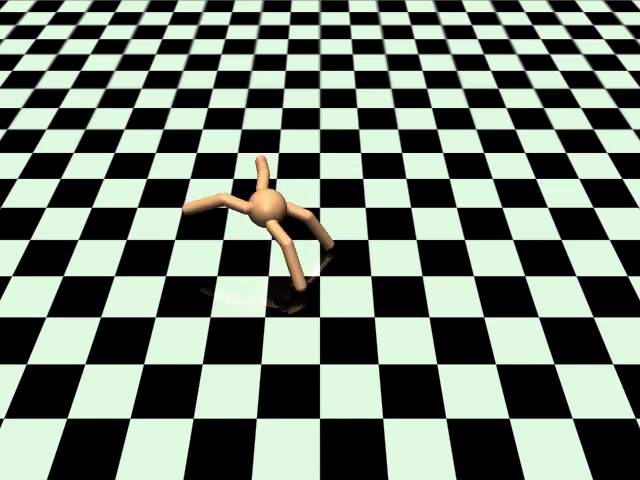
\includegraphics[width=0.5\textwidth]{images/agent_ant.png}
	\centering
	\caption{The Ant agent}\label{fig_agent_ant}
\end{figure}

\begin{figure}[H]
	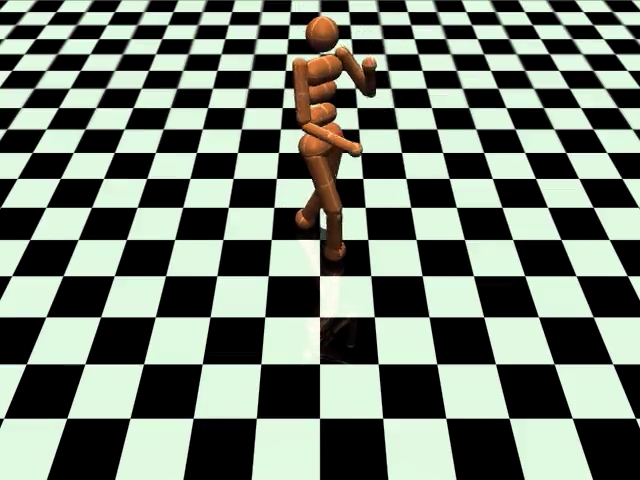
\includegraphics[width=0.5\textwidth]{images/agent_humanoid.png}
	\centering
	\caption{The Humanoid agent}\label{fig_agent_humanoid}
\end{figure}
\begin{figure}[H]
	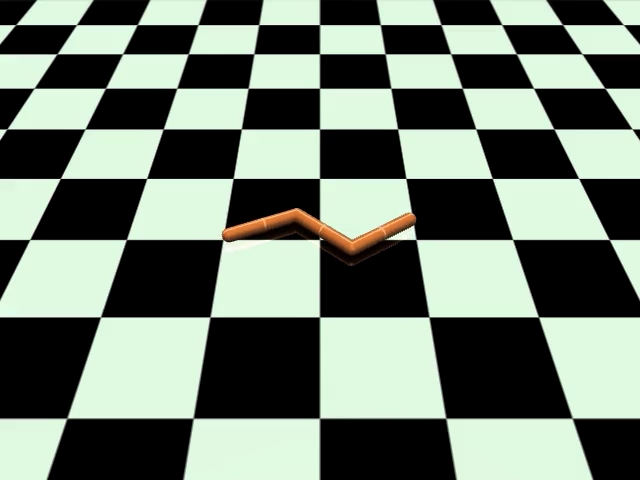
\includegraphics[width=0.5\textwidth]{images/agent_swimmer.png}
	\centering
	\caption{The Swimmer agent}\label{fig_agent_swimmer}
\end{figure}
%To provide a consistent comparison with other studies, the development of 
%!TEX program = xelatex
%!TEX root = ./thesis.tex

\subsection{Detailed Environment Specifications}
We provide a detailed description of the experiment environments in this section. All of the environments are based on the Ant task~\cite{openaigym}. 

In the original Ant task, the agent receives a 111-dimensional motion sensor input and produces an 8-dimensional action output. The input consists of a 13-dimensional vector that contains the robot's pose information, a 14-dimensional vector that represents its velocity information, and an 84-dimensional vector that contains contact force information. However, information about the agent's absolute position in the world map is not available.

For the proposed environments, the agent receives not only the 111-dimensional motion sensor input, but also a $64\times 64\times 1$ dimensional grayscale image observation. A sample image observation is shown in Figure~\ref{fig_ant_imgobs}. The image is not in a high resolution but is sufficient for the agent to observe the necessary information for the proposed tasks.

\begin{figure}[H]
	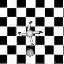
\includegraphics{images/ant_imgobs.png}
	\centering
	\caption{A sample image observation of the target environments}
\end{figure}\label{fig_ant_imgobs}

A basic task, namely move0, is similar to the Ant environment in OpenAI Gym~\cite{openaigym}. The difference is that the state space has an extra image input. The agent is required to move in a specific direction $g_0=(1,0)$, and the reward at each time-step is given by:
\begin{align}
r = v_g + 1-c_p-c_c
\end{align}
where $v_g=v \cdot g_0$ is the forward reward, which rewards the agent for moving in the target direction. A spherical object presents in the environments at a constant distance from the robot agent to represent the target direction.  $c_p$ is the control cost, which is the power that the agent is consuming, and $c_c$ is the contact cost, which penalizes the agent for collisions. The episode terminates when the agent enters the unrecoverable state of being upside-down, or if the episode length reaches 1000 time-steps.

Apart from move0, a set of similar tasks with different target directions are denoted as move1, move2, move3, ..., move7. These tasks are similar to move0 because the goal direction is different. The image observation is actually redundant for all these low-level tasks, because the agent only needs to move in one specific direction in their corresponding environments. Snapshots of these source tasks are shown in Figure~\ref{fig:task8}.
\begin{figure}[!htbp]
	\centering
	\begin{subfigure}[t]{0.3\textwidth}
		\centering
		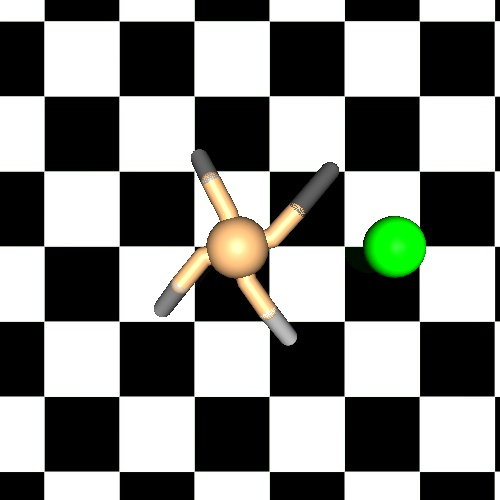
\includegraphics[width=\textwidth]{move0}
		\caption{move0}
	\end{subfigure}%
	~ 
	\begin{subfigure}[t]{0.3\textwidth}
		\centering
		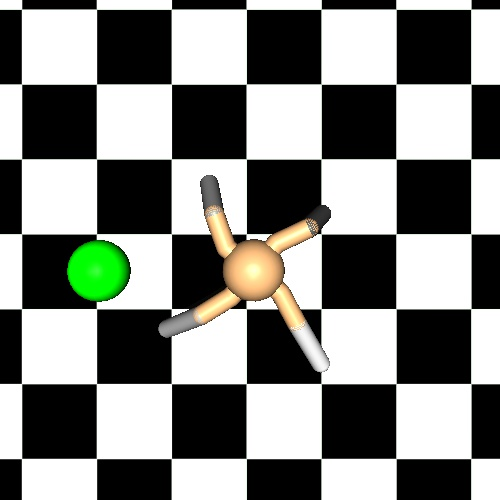
\includegraphics[width=\textwidth]{move1}
		\caption{move1}
	\end{subfigure}
	~ 
	\begin{subfigure}[t]{0.3\textwidth}
		\centering
		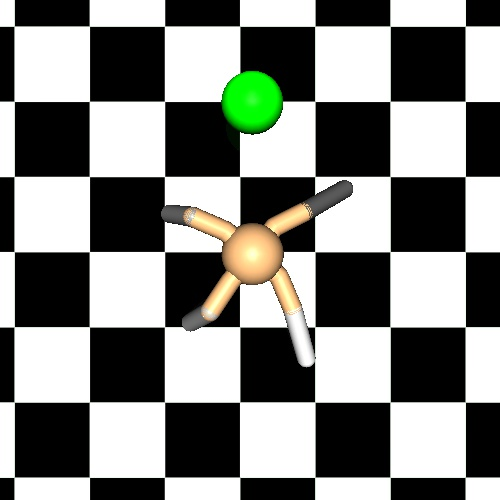
\includegraphics[width=\textwidth]{move2}
		\caption{move2}
	\end{subfigure}
	~ 
	\begin{subfigure}[t]{0.3\textwidth}
		\centering
		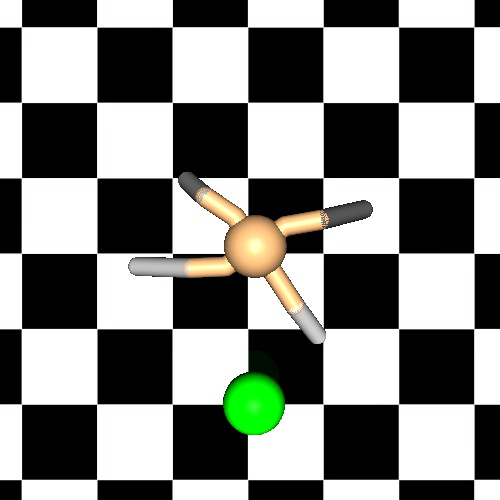
\includegraphics[width=\textwidth]{move3}
		\caption{move3}
	\end{subfigure}
	~ 
	\begin{subfigure}[t]{0.3\textwidth}
		\centering
		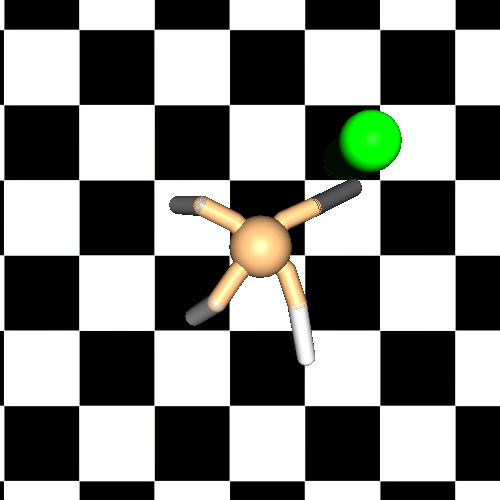
\includegraphics[width=\textwidth]{move4}
		\caption{move4}
	\end{subfigure}
	~ 
	\begin{subfigure}[t]{0.3\textwidth}
		\centering
		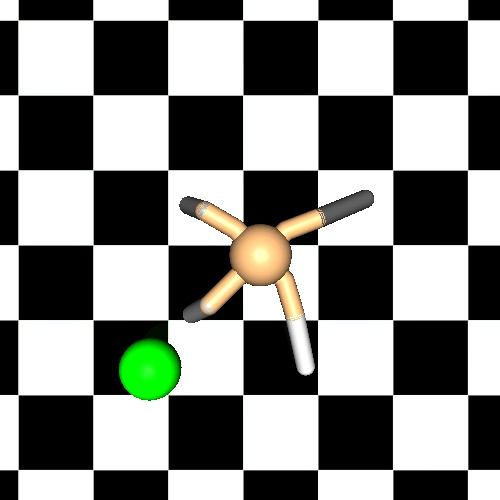
\includegraphics[width=\textwidth]{move5}
		\caption{move5}
	\end{subfigure}
	~ 
	\begin{subfigure}[t]{0.3\textwidth}
		\centering
		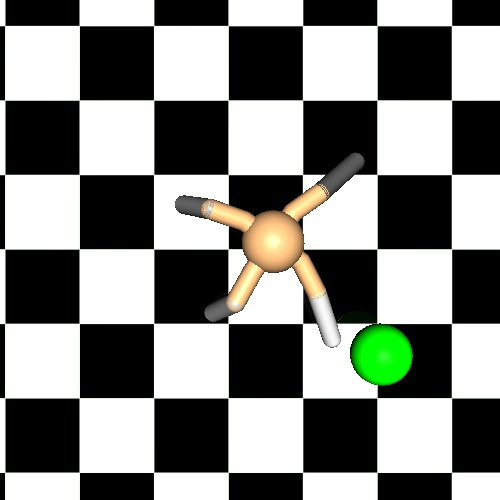
\includegraphics[width=\textwidth]{move6}
		\caption{move6}
	\end{subfigure}
	~ 
	\begin{subfigure}[t]{0.3\textwidth}
		\centering
		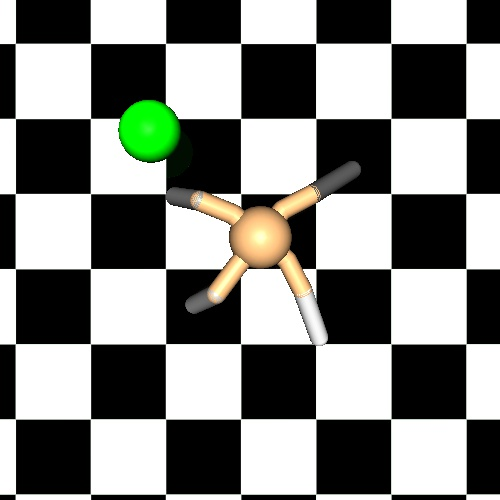
\includegraphics[width=\textwidth]{move7}
		\caption{move7}
	\end{subfigure}

	\caption{The source tasks}
	\label{fig:task8}
\end{figure}

Apart from these simple task, we also propose a set of tasks with more complexity. We propose several tasks with multi-modal state spaces such as moveg2, movecont, dynamicg8. These tasks require the agent to learn not only from the state representation but also the image representation. We also propose several more challenging tasks which has sparse reward fucntions, such as reachcont. The agent receives sparse reward signals in these environments. The target direction or location is represented by a spherical object and can be seen in the image observation.
The set of all the proposed environments are described in details in table \ref{table_ant_envs}.


\begin{table}[!htbp]

\begin{center}
\begin{tabular}{|c|p{3cm}|p{4cm}|p{4cm}|}
\hline
Task name & Goal & Reward  &  Description \\
\hline\hline
move0 & velocity: $g_0=(1,0)$ &$ v_g+1-c_p-c_c$  & move in a target direction \\
\hline
move1 & velocity: $g_1=(-1,0)$ &$ v_g+1-c_p-c_c$  & move in a target direction\\
\hline
move2 & velocity: $g_2=(0,1)$ &$ v_g+1-c_p-c_c$  & move in a target direction \\
\hline
move3 & velocity: $g_3=(0,-1)$ &$ v_g+1-c_p-c_c$  & move in a target direction \\ 
\hline 
move4 & velocity: $g_4=(\sqrt{2}/2,\sqrt{2}/2)$ &$ v_g+1-c_p-c_c$  & move in a target direction \\ 
\hline 
move5 & velocity: $g_5=(-\sqrt{2}/2,-\sqrt{2}/2)$ &$ v_g+1-c_p-c_c$  & move in a target direction \\ 
\hline 
move6 & velocity: $g_6=(\sqrt{2}/2,-\sqrt{2}/2)$ &$ v_g+1-c_p-c_c$  & move in a target direction \\ 
\hline 
move7 & velocity: $g_7=(-\sqrt{2}/2,\sqrt{2}/2)$ &$ v_g+1-c_p-c_c$  & move in a target direction \\ 
\hline 
moveg2 & velocity samples from: $\{g_0,g_1\}$ &$ v_g+1-c_p-c_c$  & each episode has a random sampled target direction \\ \hline
%moveg4 & velocity samples from: $\{g_0,g_1,g_2,g_3\}$ &$ v_g+1-c_p-c_c$  & each episode has a random sampled target direction \\ \hline
%moveg8 & velocity samples from: $\{g_0,g_1, \dots,g_7\}$ &$ v_g+1-c_p-c_c$  & each episode has a random sampled target direction \\ \hline
movecont & velocity samples from the unit circle&$ v_g+1-c_p-c_c$  & each episode has a random sampled target direction \\ \hline
dynamicg8 &  velocity samples from: $\{g_0,g_1, \dots,g_7\}$ &$ v_g$  & the target direction is re-sampled with probability 0.005 at each time-step  \\ \hline
%dynamiccont & velocity samples from a continuous range of all unit directions &$ v_g$  & the target direction is re-sampled with probability 0.005 at each time-step  \\ \hline
%reachg4 & position samples from $\{g_0,g_1,g_2,g_3\}$ & $I(\lVert x-g\rVert_2^2<0.5) - 0.01$  & The agent is terminated when reaching a target position\\ \hline
reachcont & position samples from the unit circle & $I(\lVert x-g\rVert_2^2<0.5) - 0.01$  & the episode is terminated when reaching a target position\\ \hline
reachcontreg & position samples from the unit circle & $5I(\lVert x-g\rVert_2^2<0.5) - 0.01$  & a new target is sampled and the episode continuous once the target position is reached\\ \hline
constdirreachreg & target direction samples from: $\{g_0,g_1, \dots,g_7\}$ & $5I(x_g > 1) - 0.01$  & a reward is given once the agent has moved in the target direction for a constant distance, then a new target is sampled\\ \hline
\end{tabular}
\end{center}
 \caption{Specification of the tasks}
\end{table}\label{table_ant_envs}




%!TEX program = xelatex
%!TEX root = ./thesis.tex
\section{Wasserstein Actor Critic Kronecker-factored Trust Region Policy Optimization Method }
As is reported in \cite{henderson2017matters}, the result of the current state-of-art deep reinforcement learning methods for continuous control, including TRPO, ACKTR, PPO and DDPG are difficult to be reproduced, due to they're heavily influenced by a variety of factors including random seed, neural network architecture, activation functions of neural network layers and even software implementation. This fact has reduced the reliability of these methods, and introduces difficulty in comparing their performance.

Particularly, the reproducibility problem with trust region methods including TRPO and ACKTR could be due to the training gets stuck in local minimum states. These trust region method has a naturally decreasing learning rate due to the KL-divergence measure. 

We propose a new policy optimization method, namely Wasserstein Actor Critic Kronecker-factored Trust Region Policy Optimization (W-KTR), in order to achieve a better performance on the proposed tasks, in terms of the agent's final performance, total training time and reproducibility.

The proposed W-KTR method focus on the problem scope of deep reinforcement learning for continuous control, specifically robot control problems. The physical meaning of action of these environments usually stands for mechanics-related physical quantity, such as motor torque and target motor phase. However, the traditional KL-divergence based trust region algorithms may not be suitable for these problems. Because the KL-divergence only focus on the intersection of policy distributions and may not be a good measure of the deviation of policy. A small perturbation in the mean value of a policy with Gaussian distribution from 1.0 to 1.01 will lead to a large KL-divergence when the variance has a small value such as 0.003. However, the perturbation may not lead to a significant difference in reality.

Therefore, we propose to use the Wasserstein metric, to measure the deviation of the policy updates. The Wasserstein metric as a trust region criteria has also been studied in previous literature~\cite{tolstikhin2017wasserstein}. We reformulate the trust region policy optimization problem as follows:
\begin{equation}
    \begin{aligned}
&    \underset{\theta}{\text{maximize}} 
&& J(\theta) \\
& \text{subject to } 
&& \overline{W_2}(\pi_{\theta_{old}},\pi_\theta) \leq \delta_{W}\end{aligned}
\end{equation}
where $ \overline{W_2}(\pi_{\theta_{old}},\pi_\theta)$ is the average Wasserstein-2 metric between the old policy and the current policy.

The Wasserstein-2 metric is defined by the following equation \cite{villani2003topics}:
\begin{equation}
    W_2(P,Q) = 
    \inf_{\Gamma \in \mathbb{P}(X \sim P, Y \sim Q)}
    \mathbb{E}_{X,Y \sim \Gamma} \left[ \lVert X-Y \rVert_2^2 \right]^{1/2}
\end{equation}
where $\mathbb{P}(X \sim P, Y \sim Q)$ is the set of all joint distribution of $X,Y$ with marginals $P,Q$ respectively.

Specifically, when $P$ and $Q$ are Gaussian distributions with mean $m_1,m_2$ and covariance matrix $\Sigma_1$ and $\Sigma_2$, the squared value of Wasserstein-2 distance $W_2^2(.)$ is defined as the following equation~\cite{chafai} :
\begin{equation}
    W_2^2(P,Q) = \Vert m_1-m_2\Vert_2^2 +\mathrm{Tr}\left(\Sigma_1+\Sigma_2-2(\Sigma_1^{1/2}\Sigma_2\Sigma_1^{1/2})^{1/2}\right)
\end{equation}

The problem is solved by performing gradient updates iteratively following the natural gradient with the Rianmanian metric as $W_2$ metric:

\begin{equation}
    s=H_\theta\left( \overline{W_2^2}(\pi_{old},\pi) \right)^{-1}g := A^{-1}g
\end{equation}
%
%We use the approximation of the Rianmanian metric tensor A:
%
%\begin{equation}
%    A \approx \mathbb{E}_{s_t} \left[
%    \nabla_\theta W_2^2(\pi_{old},\pi) \left(\nabla_\theta W_2^2(\pi_{old},\pi) \right)^T
%    \right]
%\end{equation}
If the non-diagonal entries in covariance matrices are all zero, the metric $W_2^2(.)$ is simply a second order term over the means and the square root of the covariance matrices:
\begin{equation}
W_2^2(P,Q) = \Vert m_1-m_2\Vert_2^2 +\Vert \Sigma_1^{1/2}-\Sigma_2^{1/2}\Vert_2^2
\end{equation}
The metric can actually be represented as a squared error between two parameter vectors:
\begin{equation}
W_2^2(P,Q) = \Vert \text{vec}[m_1,diag(\Sigma_1^{1/2})]-\text{vec}[m_2,diag(\Sigma_2^{1/2})]\Vert_2^2 
\end{equation}
The solution of this kind of expressions can then be computed using the Kronecker-factor approximation technique~\cite{wu2017scalable}.

The policy is then updated following the gradient direction $s$ with ADAM stochastic optimization algorithm~\cite{kingma2014adam}. The step size is adjusted in an adaptive manner according to the resulting $W_2$ distance at each training step.
%!TEX program = xelatex
%!TEX root = ./thesis.tex
\section{Efficient Exploration Through Exceptional Advantage Regularization}\label{sec_method_expadv_reg}
One of the challenges with multi-modal state-space robot environments is to simultaneously learn features from different sources of state inputs.

The state spaces of the studied problems have two modalities: the locomotion sensor signal and the image observation. The complexity in learning the features from the two inputs is different. The learning of motion sensor signal features is usually trivial while the learning of image features takes much more time. The agent would get stuck at a local minimum after it has learned the features of the locomotion state vectors but still without learning anything from the image input.

As far as we know, the distribution type of the continuous stochastic policy in reinforcement learning is usually chosen to be a normal distribution with diagonal covariance matrices in the previous studies of on-policy policy gradient methods. We have observed a phenomenon in the training process of policy gradient methods that, the variance of policy is extremely unlikely to be increased, even when the agent has just escaped from a local minimum. This phenomenon leads to inefficiency in exploration. Therefore, a regulation method is necessary to encourage the agent to perform exploration without hurting the reinforcement learning performance.

A conventional regularization method to encourage exploration is entropy regularization:

\begin{align}
g' = g +\beta_{ent}\nabla_\theta \mathbb{E}[ H(\pi_\theta(a|s)) ]
\end{align}
where $\beta_{ent}$ is the weight controlling the penalty on low entropies.
The entropy of a normal distribution $\mathcal{N}(\mu,\Sigma)$ is defined as:

\begin{align}
	H(\pi) =  \frac{1}{2} \ln \mathrm{det}(2\pi e \Sigma)
\end{align}

If the policy distribution is a normal distribution with diagonal covariance matrix, the entropy regularization basically introduces a constant bias to the gradient of the logarithm of variance parameters. As a result, the entropy regularization method is usually hard to tune so that the agent can efficiently perform exploration without significant degradation in the reinforcement learning performance.

We propose a novel method, namely  Exceptional Advantage Regularization, that can encourage exploration. We add a term, namely Exceptional Advantage Regularization loss (EAR), to the gradient of the variance parameters:
\begin{align}
g'_\Sigma = g_\Sigma + \beta_{ex} \mathbb{E}_{\hat{A}^{GAE}(s) > 0} \left[
\hat{A}^{GAE}(s) 
\max\left(0,\nabla_\Sigma \log \pi (a|s)\right)\right]
\end{align}
%\begin{align}
%g'_\Sigma = g_\Sigma + \beta_{exc} \mathbb{E} \left[
%	\max\left(0,I(\hat{A}^{GAE}>0) \hat{A}^{GAE} \nabla_\Sigma \log \pi (a|s)\right)\right]
%\end{align}
where $\beta_{ex} $ is the weight controlling the bias on exploration.

The EAR loss adds a bias for the positive gradients of the variance parameters of the samples with positive advantage values. By introducing the EAR loss, more importance is added to the samples with low likelihood which produce exceptionally positive advantage values. As a result, the positive experiences that are rarely encountered would be paid more attention. The problem remaining is to identify the samples with low likelihood. We simply take the positive gradients of the variance parameters with respect to the log-likelihood here to filter out the samples whose likelihoods are too high.

%!TEX program = xelatex
%!TEX root = ./thesis.tex
\section{Efficient Exploration Through Robust Concentric Gaussian Mixture Policy}
Apart from the EAR method for exploration, we propose to use an alternative probability distribution type, namely Robust Concentric Gaussian Mixture, instead of a diagonal Gaussian policy used in previous works.

The proposed policy distribution, namely Robust Concentric Gaussian Mixture (RCGM) Policy, is a mixture of two Gaussian distributions,
\begin{align}
\pi (a|s) = (1-\alpha_{ex})\mathcal{N}(\mu,\Sigma) + \alpha_{ex} \mathcal{N}(\mu,q_{ex}\Sigma)
\end{align}
where the constant $\alpha_{ex}$ is the weight of second distribution. The weight $\alpha_{ex}$ can take a value in the range of $(0,1)$, such as $0.05$, and the constant $q_{ex} \in (1,)$, for example can be $5$, controls the variance of the second deviation. The larger $q_{ex}$ is, the higher the likelihood will be in the tails of the distribution. The resulting distribution actually has the same number of trainable parameters as the first component, since both $\alpha_{ex}$ are set to fixed parameters.

The KL-divergence of two RCGM policy does not have a closed form expression even for this special case. An empirical estimation can be used to approximate the KL-divergence ~\cite{hershey2007approximat}:%TODO: fix citation
\begin{align}
KL(p, q) \approx\mathbb{E}_{x\sim p} \log [ \left(p(x)/q(x)\right) ]
\end{align}

However, an empirical estimation of the KL-divergence can still be computed based on the training samples. Apart from that, the Wasserstein-2 distance between two RCGM policy can be given by:
\begin{align}&W_2^2(\pi_{0}(a|\mu_0,\Sigma_0), \pi_{1}(a|\mu_1,\Sigma_1) =  \\ \nonumber
& \ \ \ \ (1-\alpha_{ex})
W_2^2\big(\mathcal{N}(\mu_0,\Sigma_0), \mathcal{N}(\mu_1,\Sigma_1)\big)
+ \alpha_{ex} W_2^2\big(\mathcal{N}(\mu_0,q_{ex}\Sigma_0), \mathcal{N}(\mu_1,q_{ex}\Sigma_1)\big)
\end{align}


Compared to the commonly used Diagonal Gaussian distribution, the RCGM distribution could be much more robust since it has longer tails. Therefore, it is less likely that the agent gets stuck at sub-optimal policies.


\section{Hierarchical reinforcement learning architecture}
We propose to solve the reinforcement learning problem by a two-level hierarchical model. 

The hierarchical model consists of a top-level decider agent and a set of bottom-level actuator agents. The actuator agents' policies are trained im the source task environments. 

The decider agent takes an action at every time-step. It may either decide which actuator-policy should be executed, or simply skip and continue current actuator-policy. Therefore, assume there are $n_a$ sub-policies, the action space of the root agent is an $(n_a+1)$-discrete action space.

The observation space of the root agent consists of 2 parts, original statn (motion-sensor observation, image observation) and the meta state. The meta observation state the current sub-policy being executed and the number of time-steps since the last decision has been made.

Empirically, the decider agent is parameterized by two policy networks, $\theta_s$ and $\theta_d$. The network $\theta_s$, namely switcher network, outputs a binary action that decides whether the agent should simply continue using the current acting actuator policy, or switch to another policy based on the current state. The agent

The network $\theta_d$, namely decider network, outputs an $n_a$-discrete action space, that select the acting agent

The selected leaf agent executes the corresponding sub-policy and computes the primary actions the agent should take for the original environment.

 The overalll decision-making process of the decider agent is shown in Algorithm~\ref{hrl_decision_proc}.

\begin{algorithm}
\caption{The decider agent mechanism}\label{hrl_decision_proc}
\begin{algorithmic}%[1]
\Function{deciderAct}{self,$s_t$}
\State $a_{decider} \sim \pi_{decider}(s_t)$
 \If{$a_{decider} \neq 0$}
 \State $self.currentActuator \gets self.allA
ctuators[a_{decider}-1]$
 \EndIf
\State $a_{actuator} \gets self.currentActuator.act(s_t)$
\State \Return $a_{actuator}$
\EndFunction
\end{algorithmic}
\end{algorithm}


\section{Generalized advantage estimation for hierarchical reinforcement learning agents}
We propose a generalized advantage estimation method for decider agents hierarchical reinforcement learning agents. 

Assume that a decider agent makes decisions at time $t_1,t_2,\dots$, then the execution length of the decisions are $l_i = t_{i+1} - t_i, i=1,2,\dots$.

Then the definition of reward of the decider action at $t_i$ is given by:
\begin{align}
\bar{r}_{t_i} \defeq
 \sum_{l=0}^{t_{i+1}-t_i-1}
  \gamma^l r_{t_i+l}
\end{align}

Define the TD residual $\dv_{t_i}$ for $i=0,1, \dots$by:
\begin{align}
\dv_{t_i} & \defeq -V(s_{t_i}) + \bar{r}_{t_i} + \gamma^{t_{i+1}-t_i} V(s_{t_{i+1}})
\end{align}
Then the k-step advantage estimation is given by:
\begin{alignat}{2}
\hata_{t_i}^{(1)} & \defeq   \dv_{{t_i}} 
 &&=-V(s_{t_i}) + \bar{r}_{t_i} + \gamma^{t_{i+1}-t_i} V(s_{t_{i+1}})\\
\hata_{t_i}^{(2)} 
&\defeq \dv_{t_i} + \gamma^{t_{i+1}-t_i} \dv_{t_{i+1}} 
&&= -V(s_{t_i}) +\bar{r}_{t_i} + \gamma^{t_{i+1}-t_i} \bar{r}_{t_{i+1}} + \gamma^{t_{i+2}-t_i} V(t_{i+2}) 
\hata_t^{(3)} &\defeq \dv_{t} + \gamma \dv_{t+1} + \gamma^2 \dv_{t+2} &&= -V(s_t) + r_t + \gamma r_{t+1} + \gamma^2 r_{t+2} + \gamma^3 V(s_{t+3}) \label{a3}
\end{alignat}
\begin{align}
\begin{split}
\hata_{t_i}^{(k)} 
&\defeq \sum_{d=0}^{k-1} 
\gamma^{t_{i+d}-t_i} \dv_{t_{i+d}} \\
&= -V(s_t) 
+\bar{r}_{t_i} + \gamma^{t_{i+1}-t_i} \bar{r}_{t_{i+1}} 
+ \dots 
+ \gamma^{t_{i+k-1}-t_i} \bar{r}_{t_{i+k-1}} 
+ \gamma^{t_{i+k}-t_i} V(s_{t_{i+k}})
\end{split}
\end{align}
We can define the unnormalized generalized advantage estimator as a exponentially-weighted sum of these k-step advantage estimators~\cite{schulman2015high}:
\begin{align}
\hata_{t_i}^{GAE_{unnorm}(\lambda)}
&\defeq  \hata_{t_i}^{(1)} + \lambda^{t_{i+1}-t_i}  \hata_{t_i}^{(2)} + \lambda^{t_{i+2}-t_i} \hata_{t_i}^{(3)} + \dots + \lambda^{t_{i+k-1}-t_i} \hata_{t_i}^{(k)} \nonumber \\
&=  \dv_{t_i} 
+ \lambda^{t_{i+1}-t_i} (\dv_{t_i} + \gamma^{t_{i+1}-t_i} \dv_{t_{i+1}} ) \\
&\ \ \ \ \  \ \ \ \ \ \ +\lambda^{t_{i+2}-t_i} (\dv_t + \gamma^{t_{i+1}-t_i} \dv_{t_{i+1}} + \gamma^{t_{i+2}-t_i} \dv_{t_{i+2}}) + \dots \nonumber \\
&\ \ \ \ \  \ \ \ \ \ \ +\lambda^{t_{i+k-1}-t_i}  \sum_{d=0}^{k-1} \gamma^{t_{i+d}-t_i} \dv_{t_{i+d}}\\
&= (
\dv_{t_i}  \sum_{b=0}^{k-1} \lambda^{t_{i+k-1}-t_i}
+\gamma^{t_{i+1}-t_i} \dv_{t_{i+1}} \sum_{b=1}^k \lambda^{t_{i+b}-t_i} \nonumber \\
&\ \ \ \ \  \ \ \ \ \ \ +\gamma^{t_{i+2}-t_i} \dv_{t_{i+2}} \sum_{b=2}^k \lambda^{t_{i+b}-t_i}
+\dots \\
&\ \ \ \ \  \ \ \ \ \ \ +\gamma^{t_{i+k-1}-t_i} \dv_{t_{i+k-1}} \lambda^{t_{i+k-1}-t_i})
\nonumber \\
&= \sum_{d=0}^{k-1} \dv_{t_i} \gamma^{t_{i+d}-t_i} \sum_{b=0}^{k-1} \lambda^{t_{i+b}-t_i}
\label{eq:gaelam1}
\end{align}
The normalized generalized advantage estimater is then given by:
\begin{align}
\hata_{t_i}^{GAE(\lambda)}
= \frac{\hata_{t_i}^{GAE_{unorm}(\lambda)}}{\sum_{b=0}^{k-1} \lambda^{t_{i+b}-t_i}}
\end{align}
However, the unormalized GAE estimator is usually used in practice instead of the normalized one, with a postprocessing step of batch normalization to adjust the scale of the advantages. This pratical method usually lead to large advantage scales for experience data at the beginning of the episodes and small scales for the experience data near episode ends.

